\begin{frame}{Neural Network Diagram}
\begin{center}
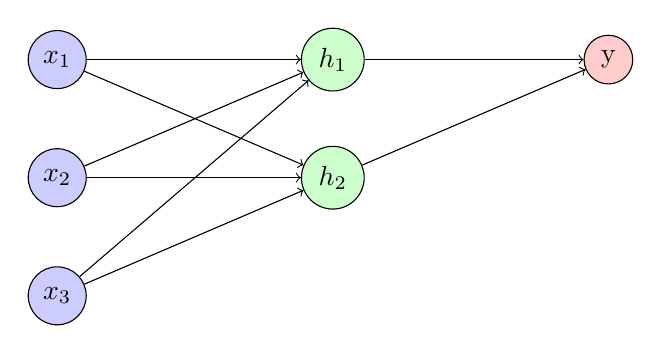
\begin{tikzpicture}[node distance=1.5cm]
    % Input layer
    \node[circle, draw, fill=blue!20] (i1) {$x_1$};
    \node[circle, draw, fill=blue!20, below of=i1] (i2) {$x_2$};
    \node[circle, draw, fill=blue!20, below of=i2] (i3) {$x_3$};
    
    % Hidden layer
    \node[circle, draw, fill=green!20, right of=i1, xshift=2cm] (h1) {$h_1$};
    \node[circle, draw, fill=green!20, below of=h1] (h2) {$h_2$};
    
    % Output layer
    \node[circle, draw, fill=red!20, right of=h1, xshift=2cm] (o1) {y};
    
    % Connections
    \draw[->] (i1) -- (h1);
    \draw[->] (i1) -- (h2);
    \draw[->] (i2) -- (h1);
    \draw[->] (i2) -- (h2);
    \draw[->] (i3) -- (h1);
    \draw[->] (i3) -- (h2);
    \draw[->] (h1) -- (o1);
    \draw[->] (h2) -- (o1);
\end{tikzpicture}
\end{center}

\footnotesize
Neural network with input, hidden, and output layers
\end{frame}